\documentclass[12pt]{article}

\usepackage{amsmath}
\usepackage[margin=0.75in]{geometry}
\usepackage[numbers]{natbib}
\usepackage{physics}
\usepackage{xcolor}
\usepackage{cancel}

\usepackage{fancyhdr}
\pagestyle{fancy}
\fancyhf{}
\rhead{Creative Destruction Lab}
\lhead{Week 2: Optimization problems \& Rydberg atom arrays}
\rfoot{Page \thepage}

\usepackage{graphicx}

\usepackage[hidelinks]{hyperref}


\renewcommand{\phi}{\varphi}

\newenvironment{changemargin}[2]{%
\begin{list}{}{%
\setlength{\topsep}{0pt}%
\setlength{\leftmargin}{#1}%
\setlength{\rightmargin}{#2}%
\setlength{\listparindent}{\parindent}%
\setlength{\itemindent}{\parindent}%
\setlength{\parsep}{\parskip}%
}%
\item[]}{\end{list}}

\title{Week 2: Optimization problems \& Rydberg atom arrays}
\author{}
\date{}


\begin{document}

\maketitle

\thispagestyle{empty}

\section*{Introduction}

Last week, you were able to simulate elements of the seminal work produced from Google's Sycamore quantum computer on your own (classical) laptops.
However, given that you are in the CDL stream, you are probably wondering how one might be able to demonstrate a quantum advantage in a ``real-world'' setting, such as optimization problems, instead of the simulatability of an ``unusual'' probability distribution (the Porter-Thomas distribution).

Superconducting-qubit (Sycamore) and trapped-ion devices are considered top contenders for scalable quantum computers, due to their long coherence times and
high gate fidelities.  However, recently neutral-atom quantum computers are also proving to be competitive due to the ease of control of a large number of programmable
qubits~\cite{serret_solving_2020,bernien_probing_2017,ebadi_quantum_2020,henriet_quantum_2020,Browaeys2020}.
%Logically, if we have access to larger quantum computers, we can foreseeably demonstrate a quantum advantage for this very reason.
Given the immense scaling solutions required for today's largest data-driven problems (e.g. supply chain management), it seems 
likely that neutral-atom quantum computers could be close close to demonstrating a quantum advantage for today's real problems.

The foundation of today's neutral-atom quantum computers is comprised of Rydberg atoms~\cite{Browaeys2020}.
Briefly, Rydberg atoms are highly-excited atoms (e.g. rubidium) that interact with each other on the scale of a few micrometres.
A controlled laser pulse can excite an atom into a quantum state with a large principal quantum number (i.e. a Rydberg state) that is quasi-stable.
The binary nature of a Rydberg atom's ground and excited states is analogous to the state of a qubit.
Besides ease of control and scalability, the value of Rydberg atoms in the context of solving real-world problems is in the way that Rydberg atoms interact with each other. 
Their interactions map trivially to a well-known mathematical problem called the Unit-Disk Maximum Independent Set (UD-MIS) problem, which is NP-hard\footnote{Problems that are NP-hard are not solvable in polynomial time, but trial solutions can be verified to be correct or not in polynomial time.}.

A host of today's real-world problems are classified as NP-hard, and it turns out that NP-hard problems can be translated into other NP-hard problems with some negligible overhead.
So, we can map a lot of real-world problems to the building blocks of quantum computers! 
This is precisely what you will be investigating this week: exploring the UD-MIS problem as it pertains to Rydberg atoms, and mapping it to a real-life NP-hard problem.
First, let's look at some of the relevant math so that you can do your tasks!

\subsection*{Modelling Rydberg atoms}

Rydberg atoms need to be placed at a physical location.
We will strictly look at Rydberg atoms on a {\it graph} $G$ with vertices (physical Rydberg atom locations) and edges $V$ and $E$, respectively.
With this, we will look at a Rydberg Hamiltonian of the form
\begin{equation} \label{eq:rydberg_hamiltonian_Omega=0}
	\hat{H} = -\sum_{i \in V} \hat{n}_i + \sum_{ i < j } \left( \frac{R_b}{r_{ij}} \right)^6 \hat{n}_i \hat{n}_j,
\end{equation}
where $\hat{n}_i = 1/2 \left( I - \hat{\sigma}_i^z \right) = \ketbra{1}{1}_i$ is called an {\it occupation operator}, $R_b$ is a parameter called the {\it blockade radius}, and $r_{ij}$ is the distance between Rydberg atoms located at vertices $i$ and $j$.
The computational basis we will be working in is the occupation basis: the eigenstates of $\hat{n}_i$,
\begin{subequations} \label{eq:occupation_basis}
    \begin{align} 
        \hat{n}_i \ket{0}_j =& 0 \qquad (\text{$\forall$ $i,j$}), \\
        \intertext{and}
        \hat{n}_i \ket{1}_j =& \delta_{i,j}\ket{1}_j,
    \end{align}
\end{subequations}
where the state $\ket{0}$ ($\ket{1}$) represents the ground (excited) state of a Rydberg atom.

On observing the form of the Hamiltonian in Eq.~\ref{eq:rydberg_hamiltonian_Omega=0}, we can see that the first term (sum over $V$) favours all sites being occupied, while the interaction term penalizes occupied pairs.
It is precisely this dichotomy that leads us to our next section.

\subsection*{Rydberg atoms and the UD-MIS problem}

The MIS problem\footnote{Not UD-MIS!} is defined as follows \cite{serret_solving_2020}: \\

\begin{changemargin}{1.5cm}{1.5cm}
	\noindent Let $G = (V,E)$ be a graph with a set of vertices $V$ and edges $E$, $N = |V|$, and $S = (n_1, \dotsb, n_N)$ be an $N$-bit string (i.e. $n_i \in 0,1$) with Hamming weight $|S| = \sum_{i = 1}^N n_i$. 
	The MIS problem is defined as finding
	\begin{align*}
		\max_{S \in \mathcal{B}} & |S|,
	\end{align*}
	subject to the constraint that $S$ is an independent set.
	Here, $\mathcal{B}$ is the set of all possible $N$-bit strings, and an independent set is defined as a set with mutually non-connected vertices: $n_i = n_j = 1 \Rightarrow (i,j) \cancel{\in} E$. \\
\end{changemargin}

Solving this problem consists of finding the largest possible independent set and returning an instance of it.
With the additional unit-disk constraint, all vertices of the given graph share an edge except those that are separated by a distance greater than 1.
An example of an independent set on a unit-disk graph is shown in Fig.~\ref{fig:udmis_example}.

\begin{figure}
    \begin{center}
        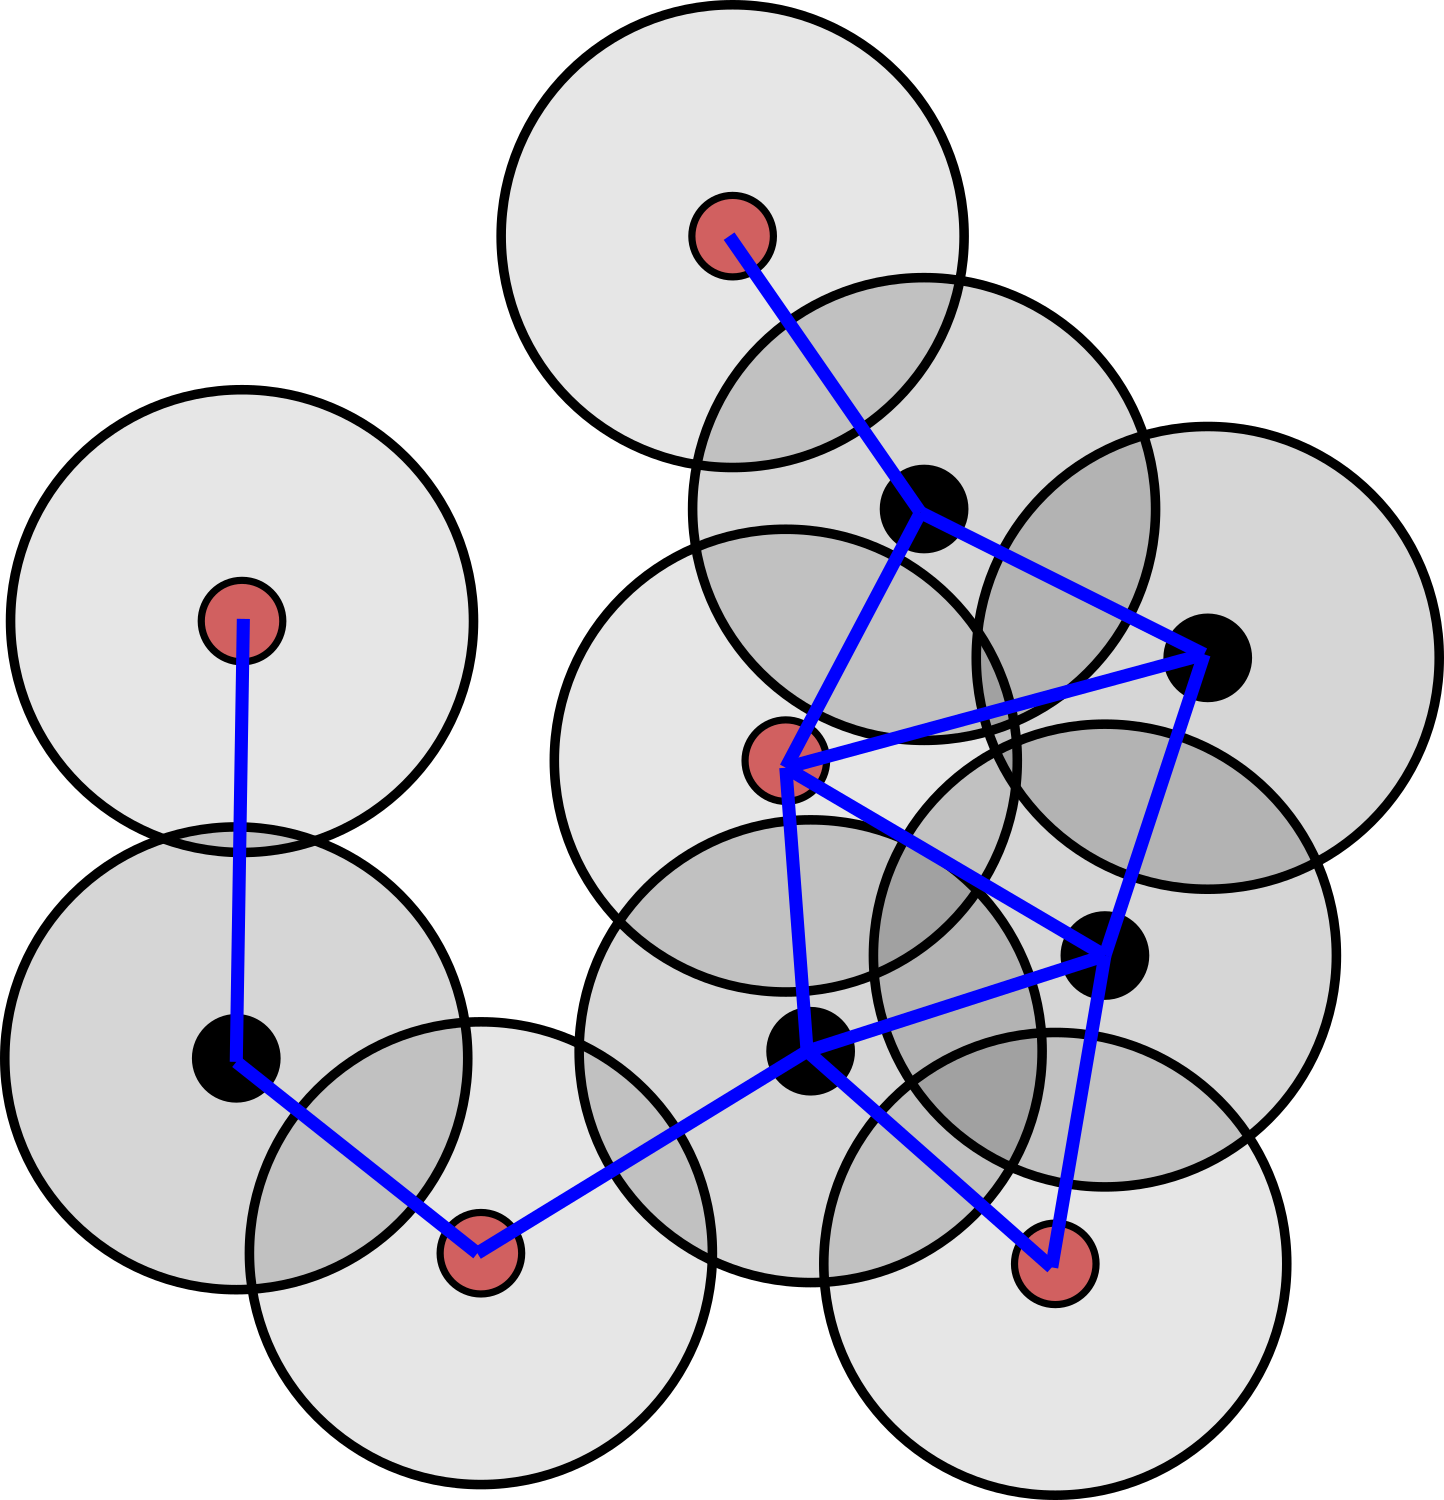
\includegraphics[width=0.4\linewidth]{images/udmis_example.png}
    \end{center}
    \caption{An example of a unit-disk graph $G$ with an instance of the corresponding solution to its UD-MIS problem. Here, blue lines indicate graph edges $E$, and dots represent vertices $V$ wherein the shaded regions represent unit-radii disks. The red dots correspond to a maximum independent set.} \label{fig:udmis_example}
\end{figure}

The ground state of the Hamiltonian
\begin{equation} \label{eq:UDMIS_hamiltonian}
	\hat{H} = -\sum_{i \in V} \hat{n}_i + u \sum_{i,j \in E} \hat{n}_i \hat{n}_j
\end{equation}
is precisely the solution to the UD-MIS problem on a graph $G$\footnote{So long as $u > 1$ \cite{serret_solving_2020}. You will use $u = 1.35$ for all of your tasks.}.
This is eerily similar to Eq.~\ref{eq:rydberg_hamiltonian_Omega=0}, with the difference being in the coefficients in front of the interaction terms.
However, to a very good approximation, it's ``similar enough''.
So, essentially, finding the ground state of a bunch of Rydberg atoms on the same graph $G$ will (approximately) solve the UD-MIS problem.

In all of your tasks, we will be modelling Eq.~\ref{eq:UDMIS_hamiltonian} for simplicity.
However, let's just take a moment to appreciate how having a physical neutral-atom quantum computer makes solving the UD-MIS problem so simple.
We could just place the Rydberg atoms at the desired vertex locations, and measure their Rydberg occupation! Pretty easy\footnote{Obviously, a lot more goes into it. These experiments are highly non-trivial affairs... No free lunch!}!

\subsection*{Task 1: Simulated Classical Annealing}

Let's first try and solve the UD-MIS problem classically.
You'll notice that the Hamiltonian in Eq.~\ref{eq:UDMIS_hamiltonian} is diagonal in the Rydberg occupation basis (Eq.~\ref{eq:occupation_basis}).
So, we can use classical Monte Carlo methods (namely the Metropolis-Hastings algorithm) to simulate this Hamiltonian at finite temperatures.
But, we're interested in the {\it ground} state, not some high-temperature state.
That being said, so long as we can simulate the Hamiltonian at a low enough temperature, it should be fine.

In this directory, you will find a Jupyter notebook titled \texttt{Task1.ipynb}.
Here, there's all the code you will need to solve the UD-MIS problem via classical {\it simulated annealing}: performing Monte Carlo simulations at lower and lower temperatures to hopefully simulate the ground (zero-temperature) state.
The {\it annealing schedule} is the manner in which the temperature is decreased.
We've provided an annealing schedule for you, but {\bf try other annealing schedules to see if you can get a solution to the UD-MIS problem faster (less steps)}.

\subsection*{Task 2: Quantum Annealing}

Let's now try solving the UD-MIS problem quantum-ly.
We will employ a quantum annealing (QA)-based approach.
Briefly, the goal of QA is to start in an easily-preparable ground state of a Hamiltonian and time evolve this state with a time-dependent Hamiltonian.
At the end of the time evolution process, the Hamiltonian should be such that its ground state is what we are after.
Consider the time-dependent Hamiltonian
\begin{equation} \label{eq:time_dep_hamiltonian}
	\hat{H}(t) = \Omega(t) \sum_{i \in V} \hat{\sigma}_i^x - \delta(t) \sum_{i \in V} \hat{n}_i + u \sum_{i,j \in E} \hat{n}_i \hat{n}_j.
\end{equation}
Notice that if $\Omega(t = 0) = \delta(t = 0) = 0$, the ground state of this Hamiltonian is every Rydberg atom in its ground state: $\ket{0}^{\bigotimes N}$.
If $\Omega(t = t_{\text{final}}) = 0$ and $\delta(t = t_{\text{final}}) = 1$, we have Eq.~\ref{eq:UDMIS_hamiltonian}.
Time-evolving the initial state $\ket{0}^{\bigotimes N}$ with the Hamiltonian in Eq.~\ref{eq:time_dep_hamiltonian} by manually choosing how to vary $\Omega(t)$ and $\delta(t)$ will hopefully give us the ground state of the UD-MIS Hamiltonian (Eq.~\ref{eq:UDMIS_hamiltonian}).
In a nutshell, this is the QA process as it pertains to our problem.

Mathematically and algorithmically, QA looks like the following
\begin{align*}
	\ket{\psi(t)} =& U(t) U(t - \delta t) \cdots U(t_0 + \delta t) U(t_0) \ket{\psi (t = t_0)},
\end{align*}
where $U(t)$ is the time-evolution operator
\begin{align*}
	U(t) =& \exp(-\frac{i}{\hbar} \delta t \hat{H}(t)),
\end{align*}
$\hat{H}(t)$ is given in Eq.~\ref{eq:time_dep_hamiltonian}, and $\delta t$ is a user-defined increment of time that defines the number of subdivisions in the time interval $t \in [t_0, t_f]$.
We will implement this on a quantum circuit simulator package in the \texttt{Julia} programming language called \texttt{Yao.jl} \cite{luo_yaojl_2020}\footnote{Created by our very own Roger Luo!}.
Everything you need is in \texttt{run\_quantum\_annealing.jl}.
We have taken inspiration from Ref.~\cite{serret_solving_2020} for the annealing schedule (see Fig. 2 in this work).
The very last line in \texttt{run\_quantum\_annealing.jl} draws samples from the resulting wavefunction $\ket{\psi(t)}$ that has been time-evolved.
{\bf Plot the samples on the graph coordinates given in the code and verify that indeed the UD-MIS problem has been solved.}

The resulting time-evolved wavefunction may not \textit{perfectly} be the ground state (i.e. when you sample it, you might get configurations that aren't the solution we desire).
Sample the resulting wavefunction several thousand times, and look for the most common bit string.
Use this as your solution\footnote{You might need to run the code a few different times!}.

\subsection*{Task 3: A Real Problem}

The City of Gotham is looking at putting in new cell phone towers.
The possible locations of the cell phone towers are given in Fig.~\ref{fig:gotham}.
The billionaire Bruce Wayne is funding the project and he loves his money. 
Therefore, Gotham should only purchase the required number of cell phone towers such that 1) the cell phone tower signal ranges do not overlap\footnote{Yes, this means some areas of Gotham City won't have cell phone service... ``Too bad,'' said Bruce.}, and 2) as much of Gotham City can be within cell signal range. 

The possible Gotham City cell phone tower locations are\footnote{All coordinates are normalized to the cell phone tower signal range.}:
\begin{enumerate}
	\item (1.19, 4.25)
	\item (2.71, 3.48)
	\item (1.19, 3.51)
	\item (2, 3.38)
	\item (1.12, 2.86)
	\item (1.70, 2.42)
	\item (2.36, 2.54)
	\item (1.52, 1.48)
	\item (2.15, 1.54)
	\item (2.14, 1.87)
	\item (1.72, 0.86)
	\item (2.29, 0.87)
\end{enumerate}

\begin{enumerate}
	\item {\bf Explain why this is a problem that can be easily mapped to the UD-MIS problem.} A few sentences is all that is needed.
	\item {\bf Solve Gotham City's problem.} Using the methods provided in Tasks 1 and 2 \textbf{Are there multiple solutions}?
	\item {\bf Should Bruce pay for a few more cell phone towers to make sure that more of Gotham City has cell phone service?}
\end{enumerate}

\begin{figure}
    \begin{center}
        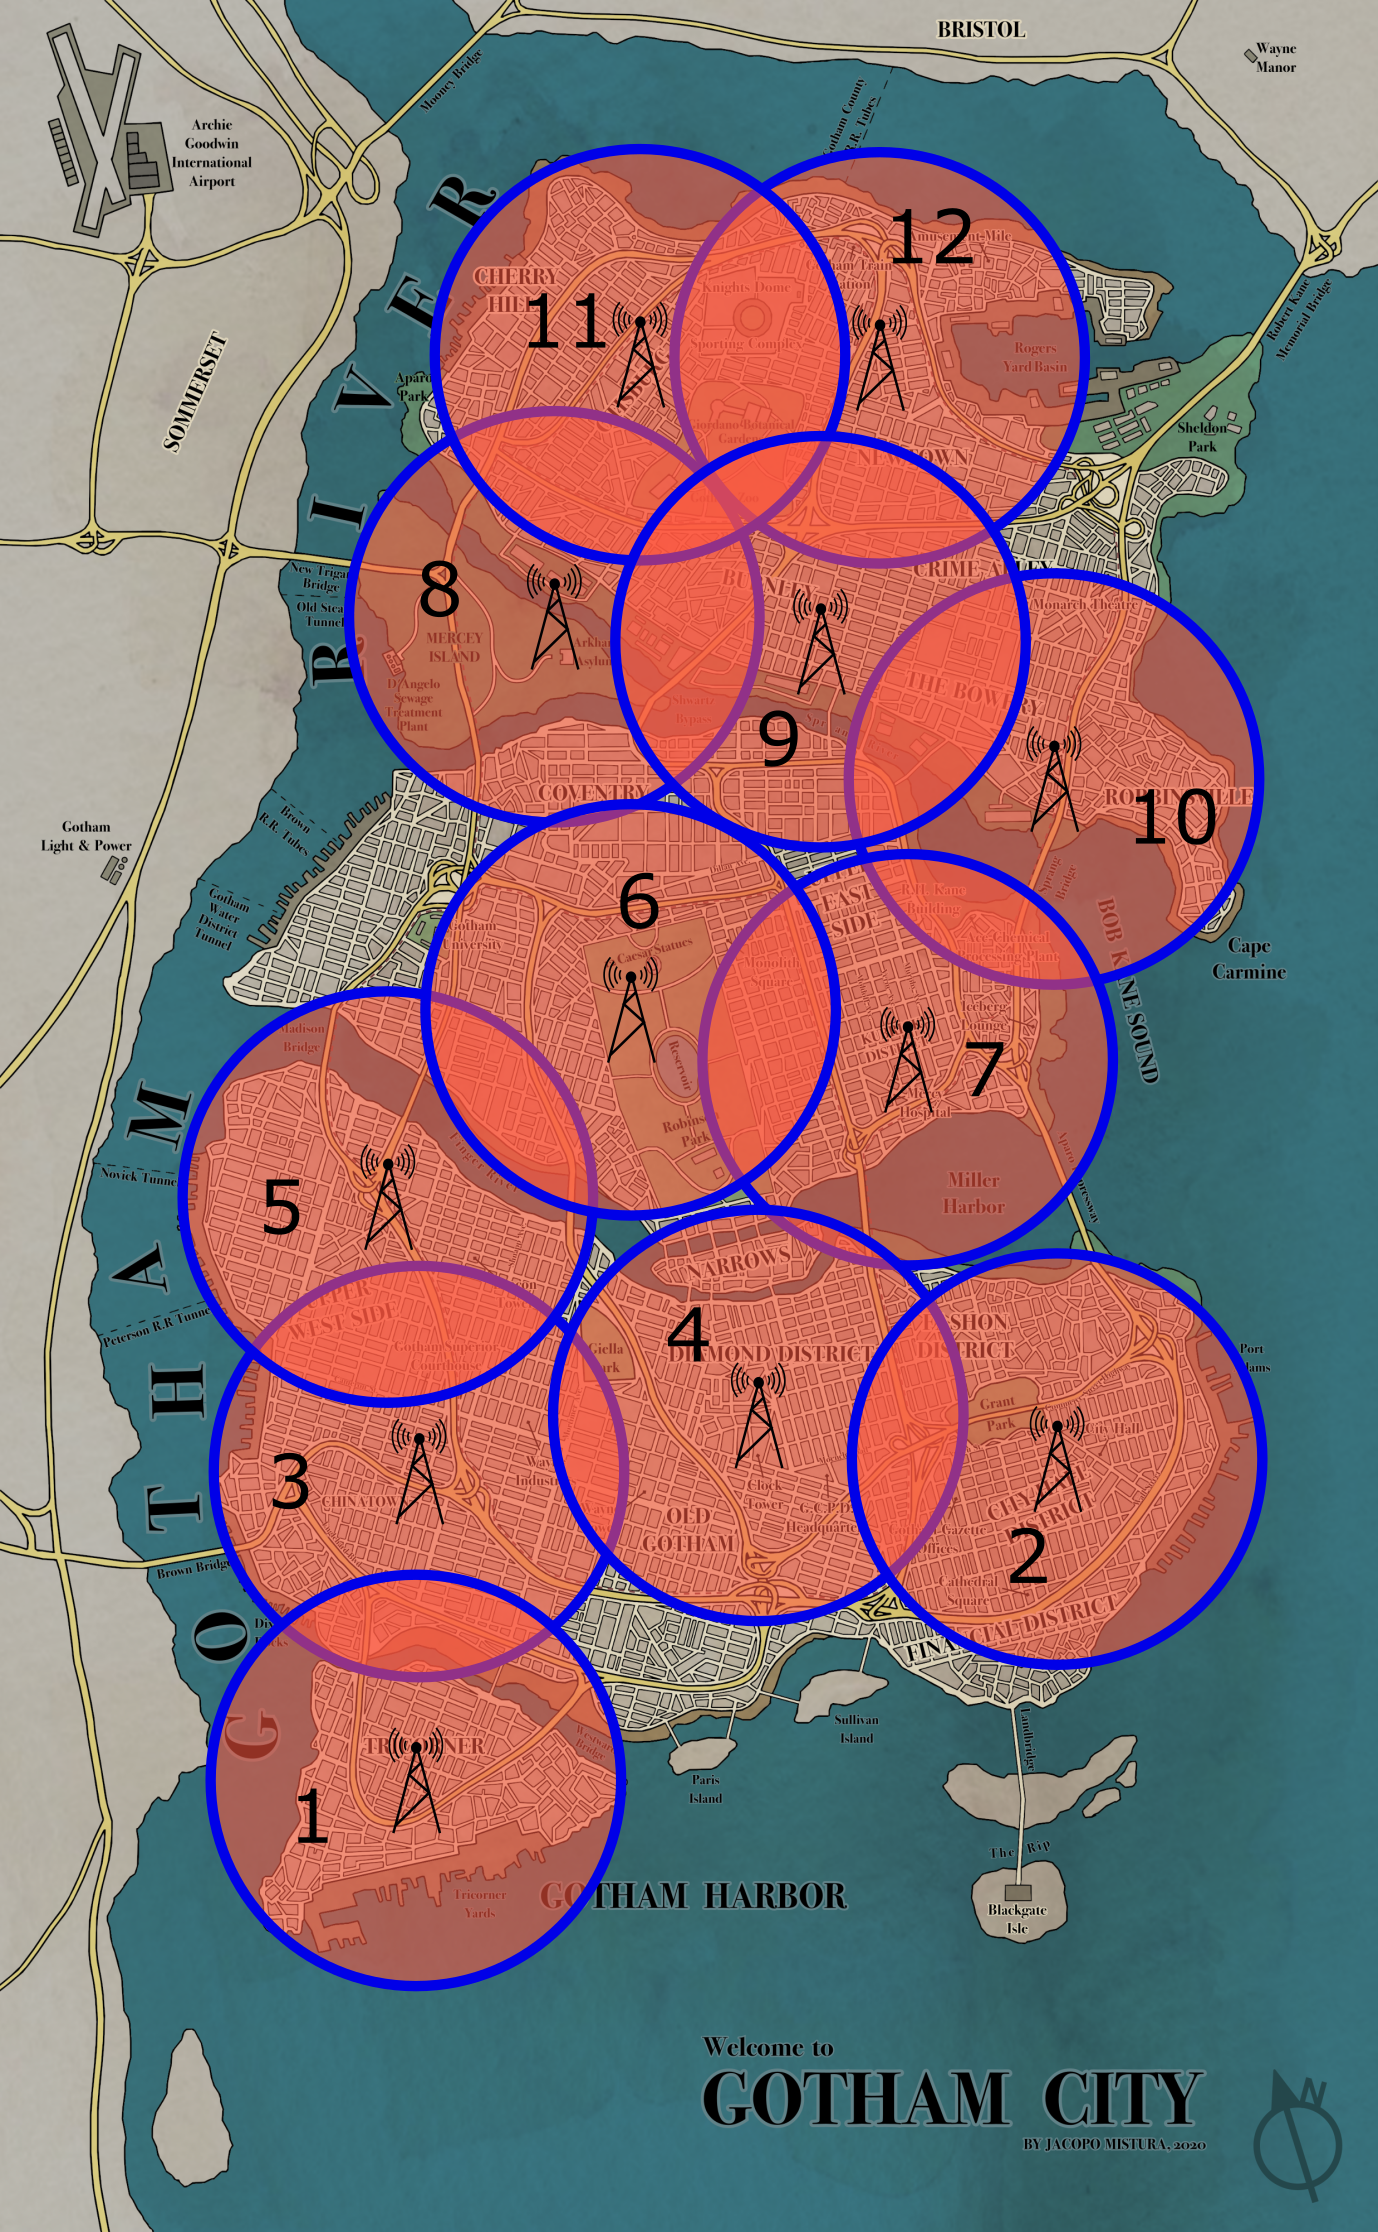
\includegraphics[width=0.4\linewidth]{images/gothamcity.png}
    \end{center}
    \caption{Possible cell phone tower locations in Gotham City.} \label{fig:gotham}
\end{figure}

\section*{Additional Challenges}

\begin{itemize}
	\item Compare / benchmark the methods outlined in the Task 1 and 2 codes.You will probably want to make larger graphs to push both of these algorithms to the test. Which method is better (i.e. faster, more efficient)?
	\item Benchmark other classical and quantum optimization methods to solve your UD-MIS problems.  
	\item Solve another real-world problem that can be mapped to the UD-MIS problem.
	\item Perform any of the tasks with real quantum hardware.

\end{itemize}

\bibliography{refs}
\bibliographystyle{unsrturl}

\end{document}
